This methodology performs a series of non-linear time history analyses (NLTHA) over one or multiple single-degree-of-freedom (SDOF) systems. In order to determine the structural capacity of the multi-degree-of-freedom (MDOF) system(s) under analysis, it is necessary to identify the relationship between the base shear and roof displacement (i.e. pushover curve). This curve should then be converted to the capacity curve of an equivalent SDOF oscillator (see Section \ref{sec:mdof_to_sdof}). For low and midrise buildings it is typically assumed that the fundamental mode of vibration corresponds to the predominant response of the structure. Under this hypothesis, the SDOF oscillator represents the first mode of response of the structure. This is usually valid for buildings with fundamental periods of vibration up to approximately 1.0 s. Otherwise, higher modes should be taken into account.\\

In this methodology the demand is represented by a set of ground motion records. The response of each structure is given by the solution of the equation of motion for an inelastic SDOF under earthquake excitation:

\begin{equation}
m\ddot{u}(t) + c\dot{u}(t) + ku(t) = p(t)
\end{equation}

Where $u$, $\dot{u}$ and $\ddot{u}$ stand for the displacement, velocity and acceleration, respectively, over time ($t$), and $p$ represents an external excitation. The nonlinear time history analysis are performed using the open-source software for structural analysis OpenSees \citep{McKennaEtAl2000}. It is important to understand the GEM Foundation does not have authorization to distribute this tool, and therefore in order to use this methodology, users are expected to download OpenSEES (http://opensees.berkeley.edu/), and allocate it in the appropriate folder (\verb=vulnerability/derivation_fragility/NLTHA_on_SDOF=).\\

Three methodologies have been implemented to perform NLTHA on SDOF systems, differing in the way the ground motion records are pre-processed before running the structural analysis and in the post-processing of the structural responses.\
The first method, called "Unscaled Records" employs unscaled ground motion records. Multiple capacity curves should be input to obtain reliable results. It should be noted that the records could also be scaled to cover high intensity measure levels, but scaling is not required by the method itself. More details about the "Unscaled Records" method can be found in Section \ref{subsec:NLTHA-unscaled}.\
The second method implements the Multiple Stripe Analysis (MSA) \citep{Jalayer2003}, in which the records are scaled to pre-defined target intensity measure levels. The MSA is suitable to assess both single and multiple structures. More details can be found in Section \ref{subsec:NLTHA-MSA}.\
Another method has been developed to derive the fragility of buildings presenting an existing level of damage. The method has been named "Double Multiple Stripe Analysis on SDOF oscillators", because it applies two nonlinear time history analyses in sequence to SDOF oscillators, in which the second one is in the format of Multiple Stripe Analysis. More details can be found in Section \ref{subsec:2MSA}.\
The three methods share the same input models for what concerns capacity curves and damage model. The description of these input is thus reported below for all the methodologies, while the definition of the ground motion records and the derivation of fragility based on the structural responses are addressed separately in Section \ref{subsec:NLTHA-unscaled}, Section \ref{subsec:NLTHA-MSA} and Section \ref{subsec:2MSA}.\\

The user has to provide one (or multiple) capacity curve, idealized by five relevant Sd-Sa points, a value of damping ratio, the period of the structure and the degree of degradation in the cyclic rule. Of these five relevant points, four are needed to represent the hysteretic behaviour of the OpenSees material (see Figure \ref{fig:backbone}); the fifth is the origin that should be also specified in the inputs for the generation of the SDOF system in the RMTK implementation. In summary, the first point corresponds to the origin (0, 0); the second couple of Sd-Sa values (ePd1, ePf1) corresponds to the yielding point of the structure, i.e. the point beyond which the structure no longer displays an elastic behaviour; the following two points, (ePd2, ePf2) and (ePd3, ePf3), are defined as any two intermediate points between the yield point and the ultimate point which can be used to represent particular structural properties, such as reduction of stiffness due to collapse of infill panels or softening behaviour due to P-delta effects; the last point (ePd4, ePf4) corresponds to the point of maximum displacement of the structure.

Pinching4 OpenSees material is employed to model the hysteretic behaviour of the SDOF oscillator. Figure \ref{fig:backbone} illustrates the input parameters for the Pinching4 one-dimensional model: a response envelope (black lines), an unload-reload path (grey lines), and three damage rules that control the evolution of these paths, as described by \citep{LowesEtAl2003}.

\begin{figure}[htb]
  \centering
      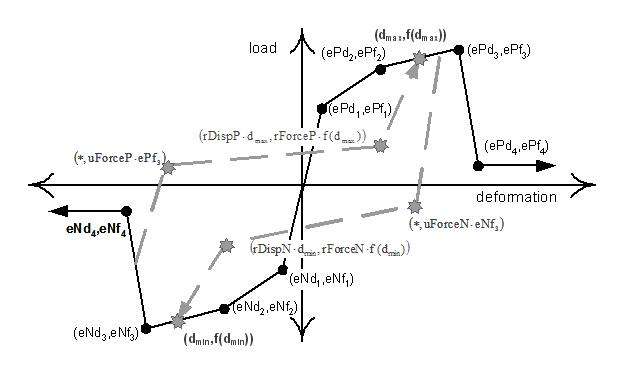
\includegraphics[width=9cm]{figures/Pinching4.jpg}
  \caption{Representation of the capacity curve required to represent the structural capacity of the SDoF system.}
  \label{fig:backbone}
\end{figure}

It can be noted that the capacity curve provided as input to the RMTK can describe only the envelope response of the hysteretic behaviour. The parameters describing the unloading and reloading path can be either user-defined or they can be set to the default values. The default values, implemented to keep the input model as simple as possible, are based on the following assumptions:\\

\begin{itemize}
\item The first assumption regards the level of pinching of the cyclic behaviour. rDispP, rForceP and uForceP (see Figure \ref{fig:backbone}) are the parameters that control the unload-reload paths of Pinching4 material; they are assigned default values of 0.5, 0.25 and 0.05, respectively to represent a medium level of pinching. Since the cyclic behaviour is considered symmetrical the parameters rDispN, rForceN and uForceN are set equal to rDispP, rForceP and uForceP, respectively.
\item The second assumption regards the degrading behaviour of the model. The parameters that control unloading, reloading stiffness and strength degradation, are gK2, gD2 and gF2, respectively. If the input parameter referring to degradation is activated (\verb=degradation= parameter set to \verb=True=) the gK2, gD2 and gF2 are assigned default values of 0.1, 0.1 and 0.4 respectively, otherwise they are set to zero and degradation is not modelled. More details about the degrading models and the meaning of the degrading parameters can be found in \citep{LowesEtAl2003} or in the OpenSees online wiki (\href{http://opensees.berkeley.edu/wiki/index.php/Pinching4_Material}{http://opensees.berkeley.edu/wiki/index.php/Pinching4\_Material}).
\end{itemize}
\\
If the User agrees with these assumptions he should set the variable \verb=sdof_hysteresis= to \verb="Default"= in the ipython notebook

\begin{Verbatim}[frame=single, commandchars=\\\{\}, samepage=true]
sdof_hysteresis = "Default"
\end{Verbatim}

If the User wants instead to define each variable of the pinching4 material himself, he should assign the variable \verb=sdof_hysteresis= the path to the file where these parameters are specified.

\begin{Verbatim}[frame=single, commandchars=\\\{\}, samepage=true]
sdof_hysteresis = "../../../../../rmtk_data/pinching_parameters.csv"
\end{Verbatim}

The pinching parameters should be defined in a csv file (tabular format) as shown in Table \ref{table:pinching4}. The variables of Table \ref{table:pinching4} are those characterising pinching4 material as explained in the OpenSees wiki (\href{http://opensees.berkeley.edu/wiki/index.php/Pinching4_Material}{http://opensees.berkeley.edu/wiki/index.php/Pinching4\_Material}). If multiple capacity curves are input, a single hysteretic behaviour can be input to describe the building class.\\

\begin {table}[htb]
\caption{Example of file containing Pinching4 material parameters}
\label{table:pinching4}
\begin{center}
  \begin{tabular}{ | c | c | c | c | c | c |}
  \hline
	rDisp  & 0.4	&	&	&	 &	\\ \hline
	fForce	 & 0.6 &	&	&	 &	\\ \hline
	uForce	 & 0	&	&	&	 &	\\ \hline
	gK1	 & 0  &	0.6  &	0  &	0	 & 1\\ \hline
	gD1	 & 0	 & 0  &	0  &	0  &	0\\ \hline
	gF1	 & 0  &	0.07	 & 0  &	0.07  &	0.9\\ \hline
	gE	 & 10 &	&	&	 &\\ \hline
	dmgType	& energy &	&	&	 &\\ \hline
	\end{tabular}
\end{center}
\end{table}			
\\
In order to use this methodology, it is necessary to specify a damage model. Currently spectral displacement, capacity curve-based and inter-storey drift-based damage criterion can be used in the damage model (see Section~\ref{subsec:dmg_model}). When the capacity curve-based criterion is selected, it may be necessary to identify the yielding spectral displacement and acceleration. The User can either input the yielding point in the input file, or he can use the algorithm described in Section \ref{subsec:cap_curves} for the idealisation of the capacity curves, to identify the spectral displacement and acceleration at yielding on the capacity curves. When inter-storey drift-based damage criterion is selected it is necessary to define a file containing the relationship between maximum inter-storey drift and spectral displacement (see Section~\ref{subsubsec:isd-dmg}). If this file is not defined a linear relationship between inter-storey drift and roof displacement is assumed and the spectral displacement is obtained dividing the roof displacement by the first modal participation factor $\Gamma$. \\

Other important inputs are the damping ratio, defined using the parameter \verb=damping=, and the degree of degradation in the hysteretic response of the SDOF system. If structural degradation wants be considered in the analysis using the default parameters, it is necessary to set the parameter \verb=degradation= to \verb=True=.

\subsection{Unscaled Records}
\label{subsec:NLTHA-unscaled}

In this method the ground motion records are unscaled and the response of each SDOF system in terms of displacement due to each ground motion record is used as input to determine the Probability Damage Matrix (PDM). The PDM represents the number of structures in each damage state per each ground motion record intensity.\
In order to use this methodology, it is necessary to load one or multiple capacity curves and a set of ground motion records, as explained in Sections \ref{subsec:cap_curves} and \ref{{subsec:gmrs} respectively. After importing the module \verb=NLTHA_on_SDOF=, it is possible to calculate the distribution of structures across the set of damage states for each ground motion record using the following command:

\begin{Verbatim}[frame=single, commandchars=\\\{\}, samepage=true]
PDM, Sds = NLTHA_on_SDOF.calculate_fragility(capacity_curves,gmrs,
damage_model,damping)
\end{Verbatim}

Where \verb=Sds= (i.e. spectral displacements) represents a vector with the maximum displacement of each structure per ground motion record and PDM is the damage probability matrix. The variable PDM can then be used to calculate the mean fragility model as described in Section \ref{subsec:derive_fragility}.

\subsection{Multiple Stripe Analysis}
\label{subsec:NLTHA-MSA}
The Multiple Stripe Analysis (MSA) consists of applying a set of ground motion records that are scaled to multiple levels of intensity measure (intensity measure bins). Multiple “stripes” of structural response are thus obtained from the SDOF oscillator subjected to the ground motion records, as depicted in Figure \ref{fig:msa}.\

\begin{figure}[htb]
  \centering
      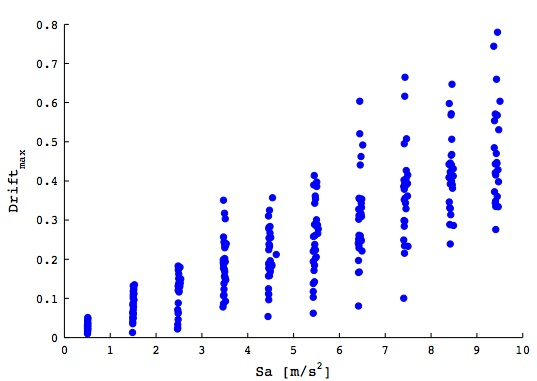
\includegraphics[width=9cm]{figures/MSA_example.jpg}
  \caption{Multiple stripes of structural responses obtained from MSA.}
  \label{fig:msa}
\end{figure}

The response of the SDOF system to each ground motion record is used to determine the Probability Damage Matrix (PDM). In this case the PDM represents the number of records leading the structure to each damage state for the intensity measure of each "stripe" of responses. With MSA it is possible to derive fragility curves also for a single structure. Alternatively more capacity curves can be input and the PDMs of the corresponding SDOF systems are summed up to get a unique PDM for the building class.

In order to to run the Multiple Stripe Analysis the User should specify the number of intensity measure bins and the number of records per bin, using the following variables:

\begin{Verbatim}[frame=single, commandchars=\\\{\}, samepage=true]
no_bins = 10
no_rec_bin = 30
\end{Verbatim}

The User should also specify the scaling factors to apply to the set of ground motion records. Another set of files is thus necessary: for each of the Intensity Measure (IM) bin a csv file must be input, containing the name of the records and the corresponding scaling factor to scale them to the given IM level. The number of records in each file should be at least equal to the number of records per intensity measure bin defined in the variable \verb=no_rec_bin=. An example of the csv file for a single intensity measure bin is given below:

\begin {table}[htb]
\caption{Example of file containing scaling factor for each ground motion record}
\label{table:scaling}
\begin{center}
  \begin{tabular}{ | c | c |}
  \hline
	IN0031xa.csv & 1.008\\ \hline
	IN0416xa.csv & 1.02\\ \hline
	IN0192xa.csv & 0.977\\ \hline
	IN0089xa.csv & 0.969\\ \hline
	IN0344xa.csv & 0.962\\ \hline
	... & ... \\ \hline
	\end{tabular}
\end{center}
\end{table}

The path to the folder where the csv files for each intensity measure bin are should be defined in the variable \verb=record_scaled_folder= (only the csv files containing the scaling factors should be in the folder) and the path to the folder where the ground motion records are should be specified in the variable \verb=gmrs_folder=, as exemplified below. The ground motion records are loaded as explained in Section \ref{subsec:gmrs}. The \verb=record_scaled_folder= contain separate csv files for the different IM bins, each file contains the name of the records and the corresponding scaling factors to scale them to the Intensity Measure of that bin. The files are then read in alphabetic order by the script, but the records indicated in each file are applied to the SDOF system in the same order in which they are listed in the file. In this way the results are "clustered" for IM bin, and they can be easily referred to the corresponding Intensity Measure Level.

\begin{Verbatim}[frame=single, commandchars=\\\{\}, samepage=true]
gmrs_folder = "../../../../../rmtk_data/MSA_records"
record_scaled_folder = "../../../../../rmtk_data/Scaling_factors"
\end{Verbatim}

After importing the module \verb=MSA_on_SDOF=, it is possible to calculate the PDM, using the following command:

\begin{Verbatim}[frame=single, commandchars=\\\{\}, samepage=true]
PDM, Sds, IML_info = MSA_on_SDOF.calculate_fragility(capacity_curves,
hysteresis, msa, gmrs, damage_model, damping_ratio, degradation)
\end{Verbatim}

Where \verb=Sds= (i.e. spectral displacements) represents a vector with the maximum displacement (of the equivalent SDoF) of each structure per ground motion record and IML$\_$info is a matrix containing the names of the ground motion records selected for the MSA and the corresponding scaling factor. The variable PDM can then be used to calculate the mean fragility model as described below.\\

First of all it is necessary to establish the intensity measure type that should be considered using the variable \verb=IMT=. Currently, the Risk Modeller’s Toolkit supports PGA, Sa, Sd and HI (Housner Intensity). If an intensity measure related to a spectral quantity is chosen, it is also necessary to establish the period of vibration (in seconds) using the variable T, and the elastic damping using the variable damping. Finally, the range of applicability of the fragility model should be defined using the variables \verb=minIML= and \verb=maxIML=.\
The results in the probability damage matrix (PDM) are used to fit a lognormal cumulative function, with a logarithmic mean ($\mu$) and logarithmic standard deviation ($\sigma$). These two parameters are calculated using one of the two currently implemented statistical methods: least squares or the maximum likelihood, selected with the variable \verb=regression_method=. An example of the required input parameters is given below:

\begin{Verbatim}[frame=single, commandchars=\\\{\}, samepage=true]
IMT = "Sa"
T = 1.5
regression_method = "max likelihood"
minIML, maxIML = 0.01, 3.00
\end{Verbatim}

The calculation of the fragility model also requires the IML$\_$info matrix (previously derived with the PDM), the set of ground motion records used in the analytical analyses (gmrs), and the damage model utilized to allocated each structure into a damage state (damage$\_$model). A description of the latter two components are provided in Section \ref{subsec:gmrs} and \ref{subsec:dmg_model}, respectively.\\
The function that calculates fragility models is contained in the module \verb=MSA_utils=. An example of this process is depicted below.

\begin{Verbatim}[frame=single, commandchars=\\\{\}, samepage=true]
fragility_model = MSA_utils.calculate_fragility_model(PDM,gmrs,
IML_info,IMT,msa,damage_model,T,damping_ratio, regression_method)
\end{Verbatim}

Once the parameters ($\mu$, $\sigma$) of the fragility model have been calculated, it is possible to save these results as explained in Section \ref{subsec:derive_fragility}.

\subsection{Double Multiple Stripe Analysis}
\label{subsec:2MSA}

The “Double MSA on SDOF Oscillators” allows performing sequences of mainshock-aftershock dynamic analyses to derive fragility curves for different levels of existing damage. The implementation of the present methodology consists of three main steps:

\begin{enumerate}
\item In the first step, unscaled ground motion records are applied to the intact structure and they are classified according to the damage state attained at the end of the nonlinear time history analysis. Once a certain number of ground motion records is found for each damage state, the dynamic analyses are stopped. If this number (pre-defined at the beginning of the analyses) is not reached, an increasing scaling factor is applied to the accelerograms until enough ground motion records populate each damage state. Finally, for each damage state, a file is generated with the corresponding list of records and the scaling factor applied. The ground motion records listed in the files are used as mainshocks of the mainshock-aftershock sequences applied in step 2.

\item In the second step, a multiple stripe analysis is performed. Each structure is led to a certain level of damage, by applying the records selected at step 1, one at the time. The structure is then subjected to another accelerogram (representative of a possible aftershock). The aftershock of the sequence is scaled to obtain a certain intensity measure level, defined at the beginning of the MSA. For each of the mainshock ground motion record the dynamic analyses are repeated for the number of records per IM level e for the number of IM levels.

\item Finally, for each initial damage state (the damage state attained after the mainshock dynamic analysis) a set of fragility curves is derived based on the results of the MSA, saved in terms of Damage Probability Matrix (DPM). The DPM is calculated allocating the structure into a damage state after each nonlinear time history analysis, and saving the defined damage state in the corresponding intensity measure bin. The number of rows of the PDM are thus equal to the number of IM bins, and the number of columns to the number of damage states.
\end{enumerate}
\\
A graphical representation of the series of analyses performed on the SDOF oscillators is depicted in Figure \ref{fig:2msa}.\

\begin{figure}[htb]
  \centering
      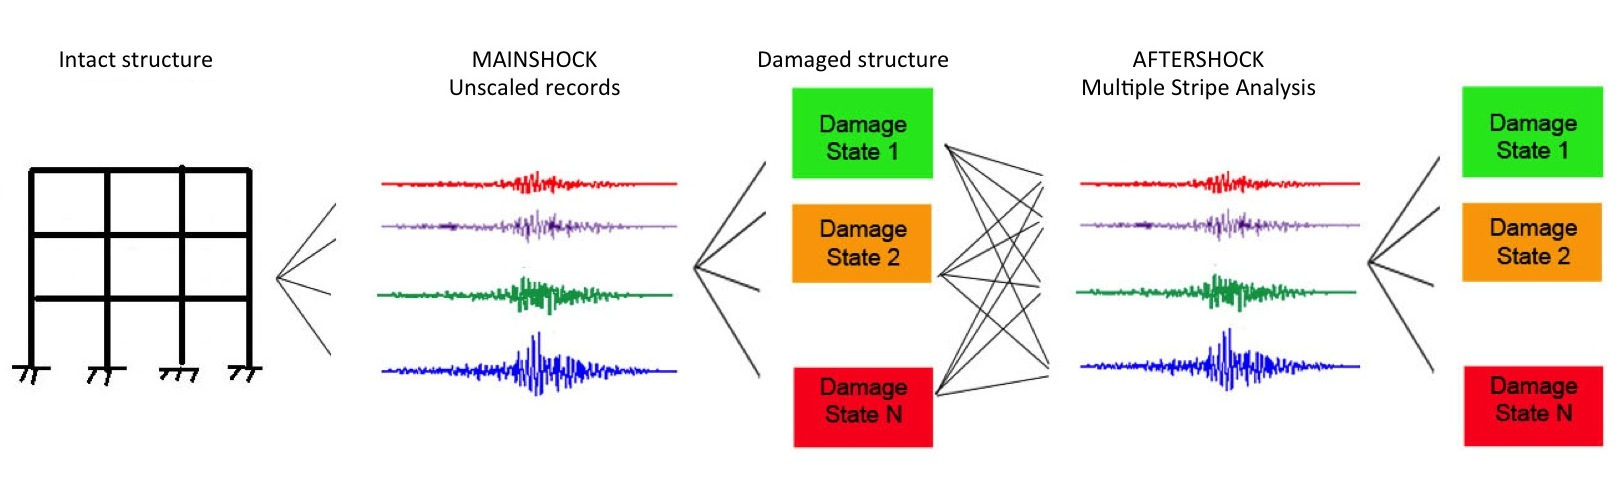
\includegraphics[width=14cm]{figures/2MSA.jpg}
  \caption{Double Multiple Stripes Analysis.}
  \label{fig:2msa}
\end{figure}

In order to use this methodology, it is necessary to load one or multiple capacity curves and a set of ground motion records, as explained in Sections \ref{subsec:cap_curves} and \ref{subsec:gmrs} respectively, while the hysteretic behaviour of the systems is set as described at the beginning of this Chapter, using the variable \verb=sdof_hysteresis=. 
It is possible to derive fragility curves for a single structure or for a building class. In the latter case many capacity curves should be input and the PDMs of the SDOF systems are summed up to get a unique PDM for the building class.
The User should also specify the number of intensity measure bins and the number of records per bin for the MSA. An essential parameter is the number of "damaged" structure to populate each initial damage state with. The following variables are thus needed:

\begin{Verbatim}[frame=single, commandchars=\\\{\}, samepage=true]
no_bins = 2
no_rec_bin = 10
number_models_in_DS = 10
\end{Verbatim}

As in the MSA described in Section \ref{subsec:NLTHA-MSA} the User should also specify the scaling factors to apply to the set of ground motion records in separate csv files for each IM bin. An example of the csv file for a single intensity measure bin is given in Table \ref{table:scaling}. The path to the folder where the csv files for each intensity measure bin are should be defined in the variable \verb=record_scaled_folder= (only the csv files containing the scaling factors should be in the folder) and the path to the folder where the ground motion records are should be specified in the variable \verb=gmrs_folder=, as exemplified below:

\begin{Verbatim}[frame=single, commandchars=\\\{\}, samepage=true]
gmrs_folder = "../../../../../rmtk_data/MSA_records"
record_scaled_folder = "../../../../../rmtk_data/Scaling_factors"
\end{Verbatim}

Moreover there is the possibility to impose a certain relationship between the ground motion characteristics of the mainshock and the aftershock of the seismic sequences. In this case the variable \verb=filter_aftershocks= should be set to \verb=TRUE= and the parameters \verb=Mw_multiplier= and \verb=waveform_path= should be defined. The former represents the ratio between the aftershock magnitude and the mainshock magnitude that wants to be imposed, the latter the path to the file containing magnitude and predominant period of each ground motion record of the selected database . More details about the relationship between mainshock and aftershock ground motion characteristics, and their use in damage-dependent fragility assessment can be found in \citep{Casotto2016}.

\begin{Verbatim}[frame=single, commandchars=\\\{\}, samepage=true]
 Mw_multiplier = 0.92
 waveform_path = '../../../../../rmtk_data/waveform.csv'
\end{Verbatim}

If the User is not interested in this option, the variable \verb=filter_aftershocks= should be set to \verb=FALSE= and the aforementioned parameters can be left empty.\\
After importing the module \verb=double_MSA_on_SDOF=, it is possible to calculate the PDM, using the following command:

\begin{Verbatim}[frame=single, commandchars=\\\{\}, samepage=true]
PDM, Sds, gmr_info = double_MSA_on_SDOF.calculate_fragility(
                        capacity_curves, hysteresis, msa, gmrs, 
                        gmr_characteristics, damage_model, 
                        damping_ratio,degradation,number_models_in_DS)
\end{Verbatim}

Where \verb=Sds= (i.e. spectral displacements) represents a vector with the maximum displacement (of the equivalent SDOF) of each structure per ground motion record of the MSA only, and \verb=IML_info= is a vector containing the names of the ground motion records selected for the MSA and the corresponding scaling factor. The variable PDM instead is a dictionary containing the PDMs for each initial damage state. It should be noted that the fragility model for each initial damage states contains information only about the higher damage states.\\ 
For each of the PDM in the dictionary the mean fragility model can be calculated as described in Section \ref{subsec:NLTHA-MSA}. The variables to be set to compute the mean fragility functions are the intensity measure type that should be considered (\verb=IMT=) the period of vibration (\verb=T=), if the intensity measure is related to a spectral quantity, and the ratio of viscous damping (\verb=damping=). Finally, the statistical method to fit the data from the PDM with a lognormal cumulative function and the range of applicability of the fragility model should be defined using the variables \verb=regression_method=, \verb=minIML= and \verb=maxIML= respectively.\

\begin{Verbatim}[frame=single, commandchars=\\\{\}, samepage=true]
IMT = "Sa"
T = 1.5
damping_ratio = 0.05
regression_method = "max likelihood"
minIML, maxIML = 0.01, 3.00
\end{Verbatim}

The calculation of the fragility model also requires the \verb=IML_info= vector (previously derived with the PDM), the set of ground motion records used in the dynamic analyses (\verb=gmrs=), and the damage model utilized to allocated each structure into a damage state (\verb=damage_model=). A description of the latter two components are provided in Section \ref{subsec:gmrs} and \ref{subsec:dmg_model}, respectively.\\
The function that calculates fragility models is contained in the module \verb=MSA_utils=. An example of this process is depicted below.

\begin{Verbatim}[frame=single, commandchars=\\\{\}, samepage=true]
fragility_model = MSA_utils.calculate_fragility_model_damaged(
PDM,gmrs,gmr_info,IMT,msa,damage_model,
T,damping_ratio, regression_method)
\end{Verbatim}

The fragility model contains the parameters ($\mu$, $\sigma$) of the fitted lognormal functions for each fin 	al damage state, for each level of initial damage. It is then possible to save these results as explained in Section \ref{subsec:derive_fragility}.